\chapter{Analysis}

\section{Introduction}
My chosen client is Michael Seamark; He is fairly experienced with working with computer systems and mainly uses a laptop to assist with his job and to surf the internet. However, he also uses an iPhone to check his emails and keep in contact with people through social networking sites.

\subsection{Define the current system}
Michael has requested that I produce a metering system which monitors gas, water and electricity consumption with several graphical outputs to represent the use and any possible savings with a way to convert between units. It should be able indicate the current cost for the consumption and predict future costs. Currently, Michael relies on the monthly bills to give him the information on his consumption of electricity, gas and water and then he has to work out any savings, calculate future costs and convert to other units if needed manually.

\subsection{Describe the problems}
One problem with the current system that Michael is using is that he cannot get the consumption of gas or electricity until the end of the month which means that he cannot check the cost of what he has used until the end of the month in which case the cost could have gone up significantly. In addition to that, the method he has to work out current spendings and future savings is inefficient and more prone to mistakes because he is calculating it manually and therefore can get values wrong or misread values from the bill 

\subsection{Section appendix}
\subsubsection{Client Interview}
\begin{enumerate}
	\item What is the proposed system required to do?
It needs to monitor energy used.you want it to monitor gas electricity accurately and be able to display the raw data in various ways eg charts so consumer can see easily what energy is being used. It will also need to calculate an average consumption for each month, 6 months and year and be able to cope with varying amounts of raw data stored in multiple units and calculate an average cost per month to calculate future costs based on the recent price and average consumption

	\item What are the problems with the current way of doing things?
The current system only monitors gas and electricity consumption and prices per month but not water and can only do one at a time so is inefficient. It is also not possible to get a reading before the month is over

	\item What data is currently recorded?
Currently only monthly gas and electricity consumption and averages for the consumption and price per month

	\item What data will the proposed system need to record?
The proposed system will need to take data on the amount of gas, electricity and water consumed per month and store. In addition to this the system will need to store averages of each for up to the past year along with prices for each month, 6 months and year and an average price for the past few months so that a prediction can be made on the cost for the coming month

	\item How will the data be recieved?
The consumption will be taken in real time and incremented onto the use for the month and the data will be stored onto a database and each month a new count will be taken along with an average price per unit of gas, electricity and water respectively

	\item What processes are performed by the current system?
The processes done by the current system are gathering daily electricity and gas consumption and adding it onto the monthly tallys, calculating a price for the past month based on the average cost per unit, calculate an average price of the past few months and calculate a predicted price for the next month

	\item What processes will the new system be required to do?
The new system will need to be able to gather daily electricity, gas and water consumption and increment it onto the monthly tallys for each one, calculate a current price of each based on the average price per unit, calculate an average price of each for the past few months, calculate the average consumption for the past few months and calculate a predicted price for the next month based on average monthly consumption on each for the past few months and average price for the past few months


	\item What algorithms do these processes use?
The current price will use an algorithm which takes the current average cost per unit for gas, electricity and water and multiply the costs by their current consumption values for each.
The average consumption will use an algorithm which calculates the sum of gas consumption for the past few months, the electricity consumption for the past few months and water consumption for the past few months and divide those sums by how many months the average taken data from. 
The average price will use an algorithm similar to the one for the average consumption but it will use values for the prices of each for the past few months rather than consumption

	\item Which processes should be executed manually?
All processes should be automated rather than be done manually

	\item What are the inputs to the current system?
The current system takes inputs for consumption for gas and electricity each day and average unit prices

	\item What inputs are required for the proposed system?
The proposed system will need to take inputs for gas, electricity and water consumption in real time and average unit prices

	\item What are the outputs from the current system?
The current system outputs an average consumption for gas and electricity for the past few months, a price for the past month for each, an average price for the past few months for each and a predicted price for the next month for each

	\item What outputs will be required from the proposed system?
The proposed system will output average consumptions for gas, electricity and water over the past few months, a price for the past month for gas, electricity and water, average costs for gas, electricity and water over the past few months, a predicted price for the following month for gas, electricity and water

\end{enumerate}

\section{Investigation}

\subsection{The current system}

\subsubsection{Data sources and destinations}
\begin{center}
\begin{tabular}{|l|l|l|l|}
	\hline
	\textbf{Source} & \textbf{Data} & \textbf{Example Data} & \textbf{Destination} \\ \hline
	Bill & Gas consumption data & Gas consumption for past month & Notebook \\ \hline
	Bill & Electricity consumption data & Electricity consumption for past month & Notebook \\ \hline
	Bill & Average price per unit for gas & 1.18 pounds/kWh & Notebook \\ \hline
 	Bill & Average price per unit for electricity & 1.34 pounds/kWh & Notebook \\ \hline
\end{tabular}
\label{tab:Data sources and destinations for the current system}
\end{center}

\subsubsection{Algorithms}
\begin{algorithm}[H]
	\caption{Price of gas consumption for the past month}
\begin{algorithmic}[H]
\SET{$gas\_price$}{$0$}
\RECEIVE{$total\_gas\_consumption$}
\RECEIVE{$average\_price\_per\_unit$}
\SET{$gas\_price$}{$total\_gas\_consumption * average\_price\_per\_unit$}
\SEND{$gas\_price$}
\end{algorithmic}
\end{algorithm}

\begin{algorithm}[H]
	\caption{Price of electricity consumption for the past month}
\begin{algorithmic}[H]
\SET{$electricity\_price$}{$0$}
\RECEIVE{$total\_electricity\_consumption$}
\RECEIVE{$average\_price\_per\_unit$}
\SET{$electricity\_price$}{$total\_electricity\_consumption * average\_price\_per\_unit$}
\SEND{$electricity\_price$}
\end{algorithmic}
\end{algorithm}

\begin{algorithm}[H]
	\caption{Average price of gas consumption for the past few months}
\begin{algorithmic}[H]
\SET{$average\_monthly\_price$}{0}
\SET{$total\_price$}{0}
\SEND{$"How\ many\ months\ would\ you\ like\ to\ get\ an\ average\ for?"$}
\RECEIVE{$amount\_of\_months$}
\For{$count$}{$amount\_of\_months$}
	\RECEIVE{$gas\_price$}
	\SET{$total\_price$}{$total\_price + gas\_price$}
\EndFor
\SET{$average\_monthly\_price$}{$total\_price / amount\_of\_months$}
\SEND{$average\_monthly\_price$}
\end{algorithmic}
\end{algorithm}

\begin{algorithm}[H]
	\caption{Average gas consumption for the past few months}
\begin{algorithmic}[H]
\SET{$average\_monthly\_consumption$}{0}
\SET{$total\_consumption$}{0}
\SEND{$"How\ many\ months\ would\ you\ like\ to\ get\ an\ average\ for?"$}
\RECEIVE{$amount\_of\_months$}
\For{$count$}{$amount\_of\_months$}
	\RECEIVE{$gas\_consumption$}
	\SET{$total\_consumption$}{$total\_consumption + gas\_consumption$}
\EndFor
\SET{$average\_monthly\_consumption$}{$total\_consumption / amount\_of\_months$}
\SEND{$average\_monthly\_price$}
\end{algorithmic}
\end{algorithm}

\begin{algorithm}[H]
	\caption{Average price of electricity consumption for the past few months}
\begin{algorithmic}[H]
\SET{$average\_monthly\_price$}{0}
\SET{$total\_price$}{0}
\SEND{$"How\ many\ months\ would\ you\ like\ to\ get\ an\ average\ for?"$}
\RECEIVE{$amount\_of\_months$}
\For{$count$}{$amount\_of\_months$}
	\RECEIVE{$electricity\_price$}
	\SET{$total\_price$}{$total\_price + electricity\_price$}
\EndFor
\SET{$average\_monthly\_price$}{$total\_price / amount\_of\_months$}
\SEND{$average\_monthly\_price$}
\end{algorithmic}
\end{algorithm}

\begin{algorithm}[H]
	\caption{Average electricity consumption for the past few months}
\begin{algorithmic}[H]
\SET{$average\_monthly\_consumption$}{0}
\SET{$total\_consumption$}{0}
\SEND{$"How\ many\ months\ would\ you\ like\ to\ get\ an\ average\ for?"$}
\RECEIVE{$amount\_of\_months$}
\For{$count$}{$amount\_of\_months$}
	\RECEIVE{$electricity\_consumption$}
	\SET{$total\_consumption$}{$total\_consumption + electricity\_consumption$}
\EndFor
\SET{$average\_monthly\_consumption$}{$total\_consumption / amount\_of\_months$}
\SEND{$average\_monthly\_price$}
\end{algorithmic}
\end{algorithm}

\begin{algorithm}[H]
	\caption{Predicted gas consumption price for the coming months}
\begin{algorithmic}[H]
\SET{$predicted\_cost$}{0}
\RECEIVE{$average\_gas\_consumption$}
\RECEIVE{$average\_cost\_per\_unit$}
\SET{$predicted\_cost$}{$average\_gas\_consumption * average\_cost\_per\_unit$}
\SEND{$predicted\_cost$}
\end{algorithmic}
\end{algorithm}

\begin{algorithm}[H]
	\caption{Predicted electricity consumption price for the coming months}
\begin{algorithmic}[H]
\SET{$predicted\_cost$}{0}
\RECEIVE{$average\_electricity\_consumption$}
\RECEIVE{$average\_cost\_per\_unit$}
\SET{$predicted\_cost$}{$average\_electricity\_consumption * average\_cost\_per\_unit$}
\SEND{$predicted\_cost$}
\end{algorithmic}
\end{algorithm}

\subsubsection{Data flow diagram}
\begin{figure}[H]
    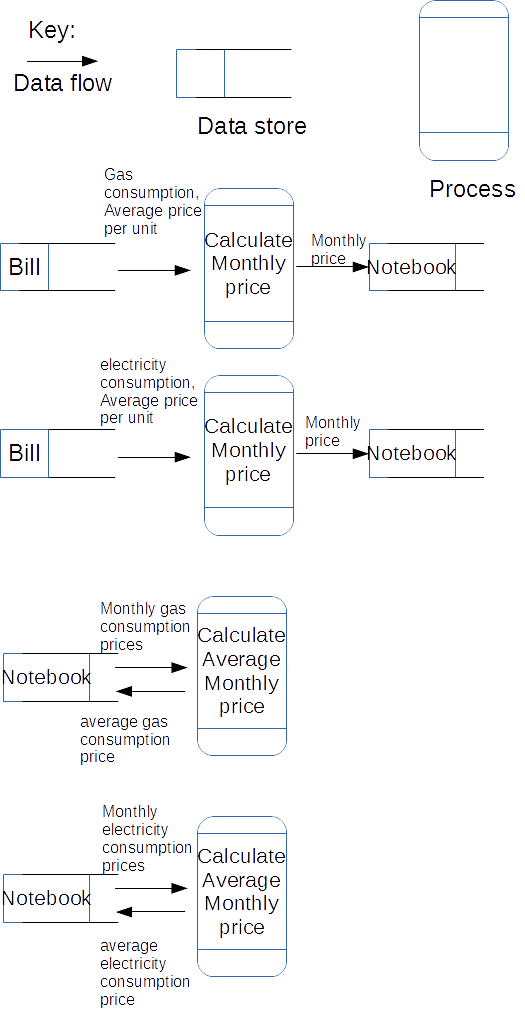
\includegraphics[width=\textwidth]{./dataflowdiagrams1.png}
    \caption{data flow diagrams for current system} \label{fig:dataflowdiagrams}
\end{figure}

\begin{figure}[H]
    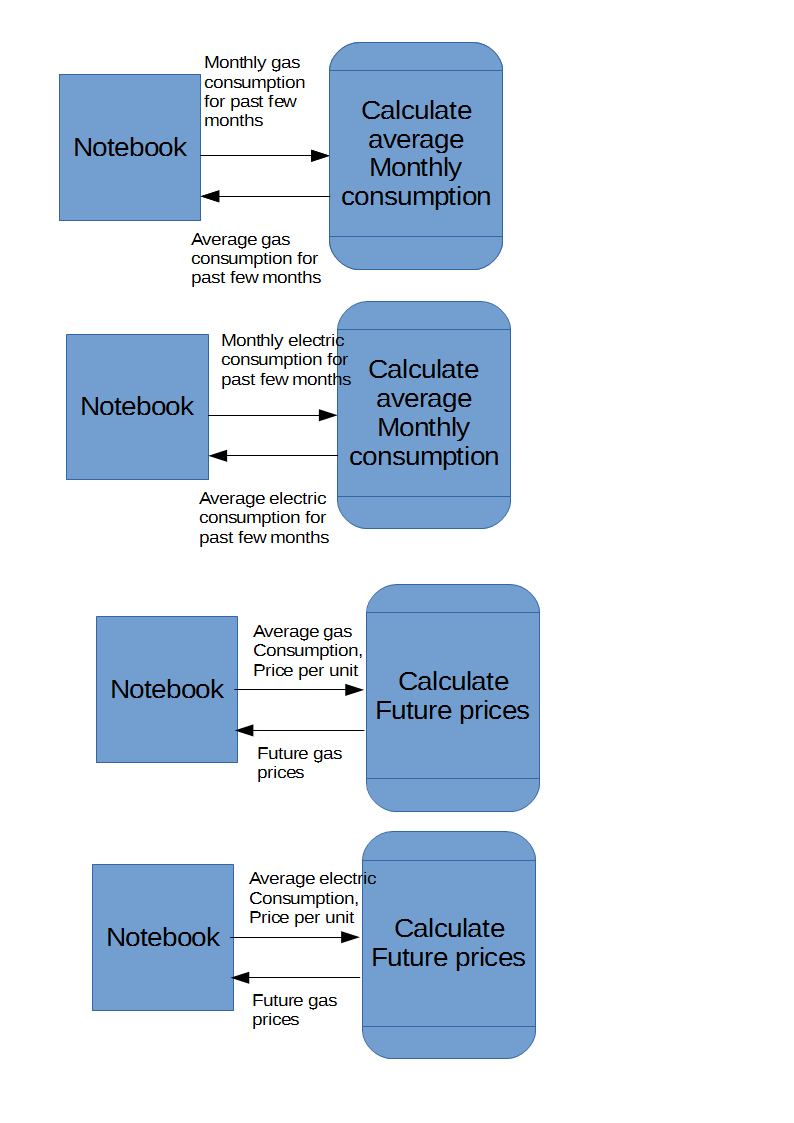
\includegraphics[width=\textwidth]{./dataflowdiagrams2.png}
    \caption{data flow diagrams for current system} \label{fig:dataflowdiagrams}
\end{figure}

\subsubsection{Input Forms, Output Forms, Report Formats}
\begin{figure}[H]
    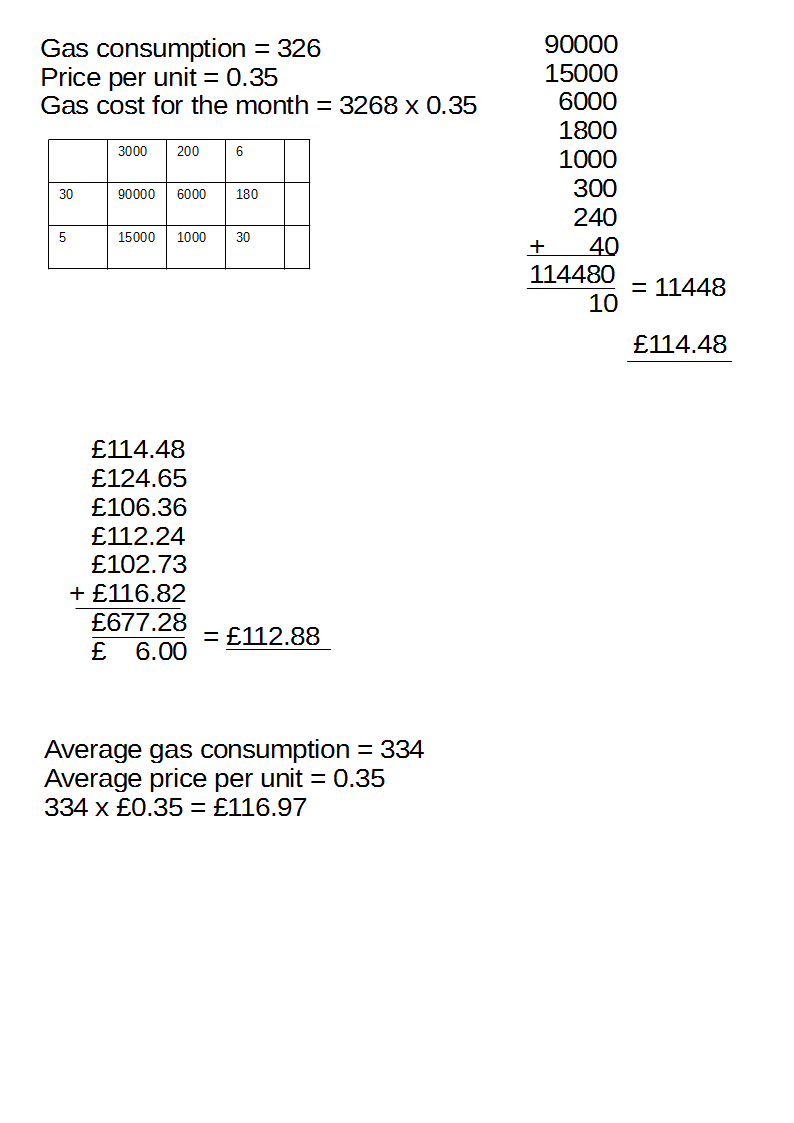
\includegraphics[width=\textwidth]{./maths.png}
    \caption{calculations for the price of one month, the average price for 6 months and a prediction for the next month} \label{fig:calculations}
\end{figure}
\subsection{The proposed system}

\subsubsection{Data sources and destinations}
\begin{center}
\begin{tabular}{|l|l|l|l|}
	\hline
	\textbf{Source} & \textbf{Data} & \textbf{Example Data} & \textbf{Destination} \\ \hline
	gas meter & gas consumption data & gas consumption & database \\ \hline
 	electricity meter & electric consumption data & electric consumption & database \\ \hline
	water meter & water consumption data & water consumption & database \\ \hline
	User input & Average price per unit for gas & 1.18 pounds/kWh & database \\ \hline
 	User input & Average price per unit for electricity & 1.34 pounds/kWh & database \\ \hline
	User input & Average price per unit for water & 1.25 pounds/litre & database \\ \hline
\end{tabular}
\label{tab:Data sources and destinations for the proposed system}
\end{center}

\subsubsection{Data flow diagram}
\begin{figure}[H]
    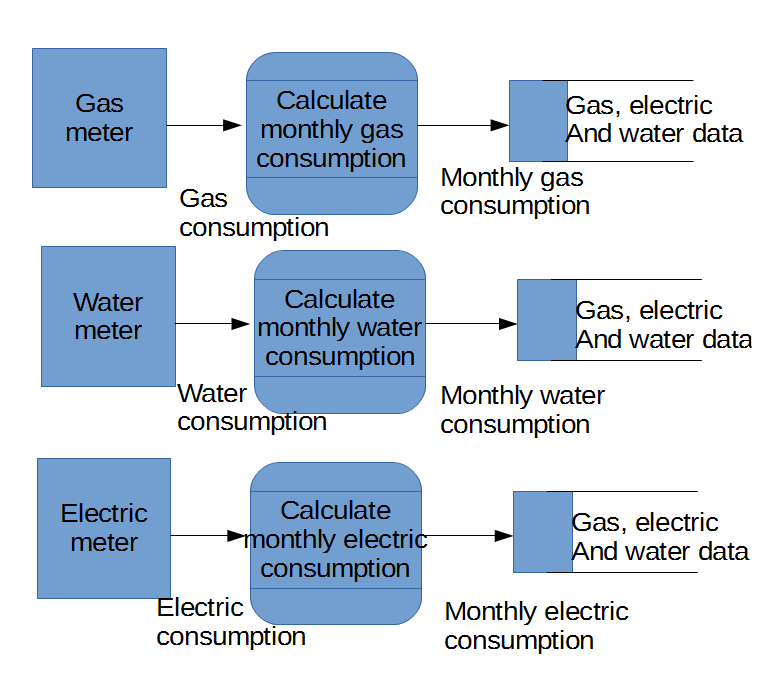
\includegraphics[width=\textwidth]{./dataflowdiagrams3.png}
    \caption{data flow diagrams for proposed system} \label{fig:dataflowdiagrams}
\end{figure}

\begin{figure}[H]
    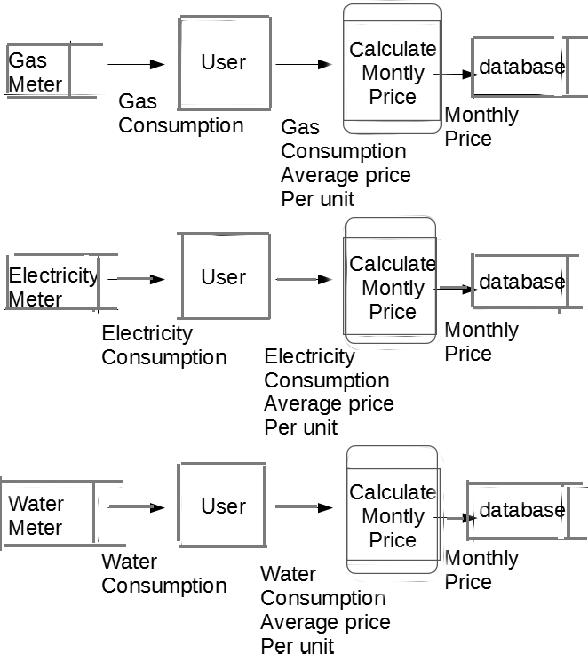
\includegraphics[width=\textwidth]{./dataflowdiagrams4.png}
    \caption{data flow diagrams for proposed sysem} \label{fig:dataflowdiagrams}
\end{figure}

\subsubsection{Data dictionary}
\begin{center}
\begin{tabular}{|p{3cm}|p{1cm}|p{1.5cm}|p{3cm}|p{2cm}|p{3.5cm}|}
	\hline
	\textbf{name} & \textbf{data type} & \textbf{length} & \textbf{validation} & \textbf{example data} & \textbf{comment} \\ \hline
	GasID & Integer & 1 - 255 & must be between 1 and 255 & 23 &  \\ \hline
	ElectricID & Integer & 1 - 255 & must be between 1 and 255 & 23 &  \\ \hline
	WaterID & Integer & 1 - 255 & must be between 1 and 255 & 23 &  \\ \hline
	GasConsumption & Double & 1-9000 & must be greater than 0 & 256.743 & value can be in multiple units \\ \hline
	ElectricConsumption & Double & 1-9000 & must be greater than 0 & 452.534 &  \\ \hline
	WaterConsumption & Double & 1-9000 & must be greater than 0 & 537.322 &  \\ \hline
	GasCostPernit & Double & 0-10 & must be between 0 and 10 & 1.53 & value is in pounds \\ \hline
	ElectricCostPerUnit & Double & 0-10 & must be between 0 and 10 & 1.42 &  \\ \hline
	WaterCostPerUnit & Double & 0-10 & must be between 0 and 10 & 1.42 &  \\ \hline
	GasCostForLastMonth & Double & 0-1000 & must be greater than 0 & 532.533 & value is in pounds \\ \hline
	ElectricCostForLastMonth & Double & 0-1000 & must be greater than 0 & 412.176 &  \\ \hline
	WaterCostForLastMonth & Double & 0-1000 & must be greater than 0 & 164.865 &  \\ \hline
	AverageGasConsumptionForPastMonths & Double & 0 - 9000 & must be a value greater than 0 & 211.431 & value can be in multiple units \\ \hline
	AverageElectricConsumptionForPastMonths & Double & 0-9000 & must be a value greater than 0 & 542.134 &  \\ \hline
	AverageWaterConsumptionForPastMonths & Double & 0-9000 & must be a value greater than 0 & 322.533 & \\ \hline
\end{tabular}
\end{center}
\subsubsection{Volumetrics}
I have chose to use an initial size of 200 records. I have chose this amount because my client said he would like to be able to check an average cost for gas, water and electric consumption for the past year and this size will allow for individual records for each month for gas, electric and water consumption for 12 months. This is a good size because it will mean that there can be average checks for any amount of months upto 12 months and the size can be expanded later on if needed. It also means I will have space to store average consumption and price for gas, electricity and water, predicted costs and consumption for coming months for gas, electricity and water and an average price per unit for recent months for gas, electricity and water. Each record for gas, electricity and water will store the details for consumption, price and average cost per unit for that month. The records for average values for gas, electricity and water will store the details of the average cost or consumption per month and how many months this is for.

The monthly records database will hold 4 data fields,with the 3 main data fields taking up 8 bytes of storage and the fourth taking up 1 byte, for each record for gas, electricity and water, which would equal a total of 108 data fields, along with an extra 3 data fields in the average values records for gas, electricity and water, two taking up 8 bytes of storage and the other field taking up 1 byte of storage. This means that the minimum amount of space needed for the database would be:

33B * 108 = 3564B
17B * 9 = 153B

3564B + 164B = 3717B
3717B / 1024 = 3.63KB

\section{Objectives}

\subsection{General Objectives}
The general objectives for the proposed system are:
\begin{itemize}
	\item Clear and easy to use menu interface for selecting what to check
	\item Clear and easy to use input and output structure for each of the consumption and price records
\end{itemize}
\subsection{Specific Objectives}
\begin{itemize}
	\item real time gathering of gas, electricity and water consumption
	\item automate as much of the system as possible
	\item output consumption data and average data into a range of units and in different output styles such as tables and graphs 
	\item predictions and averages for gas, electricity and water consumption to be done for one month, six months and one year intervals on request
	\item predictions and averages for gas, electricity and water consumption prices to be done for one month, six months and one year intervals on request
\end{itemize}
\subsection{Core Objectives}
\begin{itemize}
	\item working out averages for gas, electricity and water consumption
	\item working out averages for gas, electricity and water consumption prices
	\item working out predicted future costs for gas, electricity and water consumption
	\item working out predicted future consumption rates for gas, electricity and water
\end{itemize}
\subsection{Other Objectives}
\begin{itemize}
	\item gas, electricity and water consumptions for each day to be added to the total for each month
\end{itemize}
\section{ER Diagrams and Descriptions}

\subsection{ER Diagram}
\begin{figure}[H]
    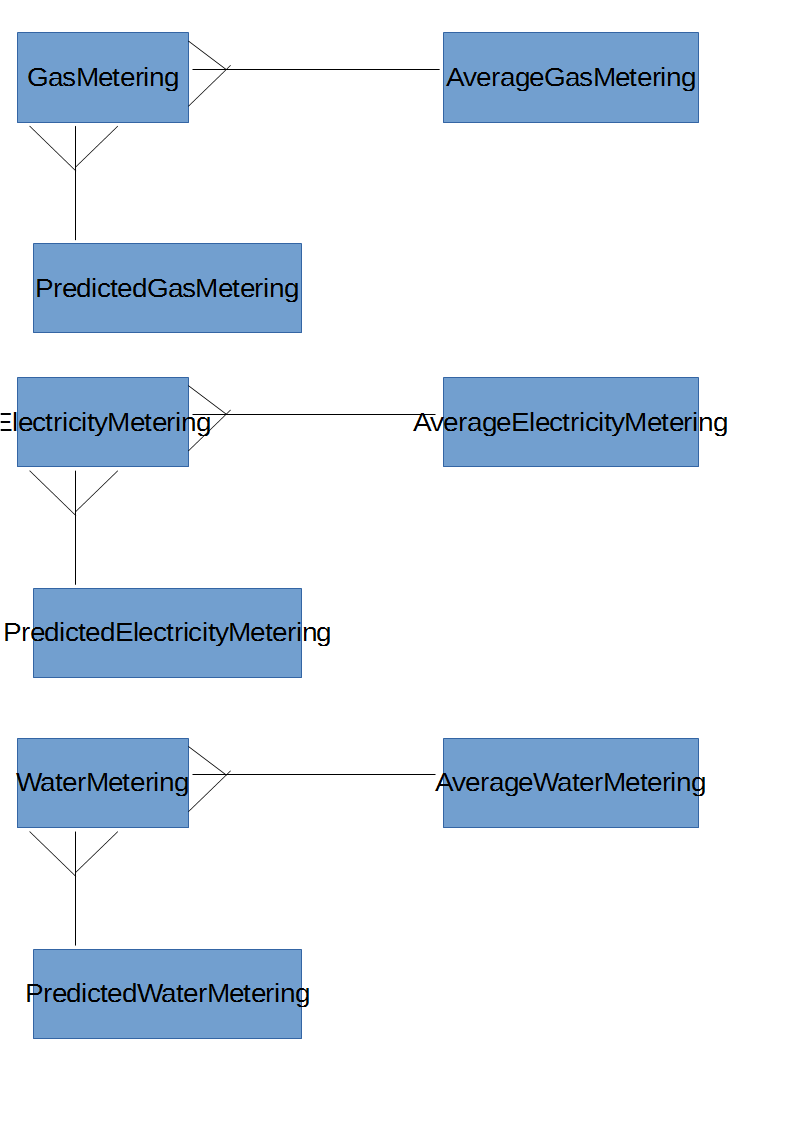
\includegraphics[width=\textwidth]{./ERDiagram.png}
    \caption{ER Diagrams for the proposed system} \label{fig:ER Diagrams}
\end{figure}
\subsection{Entity Descriptions}
	GasMetering(\emph{GasID},Consumption, Price, PricePerUnit, UnitType)\\
	ElectricityMetering(\emph{ElectricityID}, Consumption, Price, PricePerUnit)\\
	WaterMetering(\emph{WaterID}, Consumption, Price, PricePerUnit)\\
	AverageGasMetering(\emph{AverageGasID}, AverageConsumption, AveragePrice)\\
	AverageElectricityMetering(\emph{AverageElectricityID}, AverageConsumption, AveragePrice)\\
	AverageWaterMetering(\emph{AverageWaterID}, AverageConsumption, AveragePrice)\\
	PredictedGasMetering(\emph{PredictedGasID}, PredictedConsumption, PredictedPrice)\\
	PredictedElectricityMetering(\emph{PredictedElectricityID}, PredictedConsumption, PredictedPrice)\\
	PredictedWaterMetering(\emph{PredictedWaterID}, PredictedConsumption, PredictedPrice)\\
\section{Object Analysis}

\subsection{Object Listing}
\begin{itemize}
	\item GasMetering
	\item ElectricityMetering
	\item WaterMetering
	\item AverageGasMetering
	\item AverageElectricityMetering
	\item AverageWaterMetering
	\item PredictedGasMetering
	\item PredictedElectricityMetering
	\item PredictedWaterMetering
\end{itemize}
\subsection{Relationship diagrams}
\begin{figure}[H]
    \includegraphics[width=\textwidth]{./Relationships.png}
    \caption{Relationship Diagrams for the proposed system} \label{fig:Relationship Diagrams}
\end{figure}
\subsection{Class definitions}
\begin{figure}[H]
    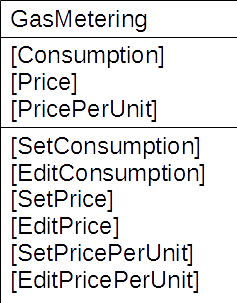
\includegraphics[width=\textwidth]{./GasMetering.png}
    \caption{Class Diagrams for the proposed system} \label{fig:GasMetering Class Diagram}
\end{figure}
\begin{figure}[H]
    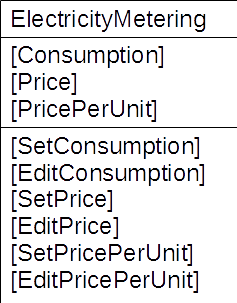
\includegraphics[width=\textwidth]{./ElectricityMetering.png}
    \caption{Class Diagrams for the proposed system} \label{fig:ElectricityMetering Class Diagram}
\end{figure}
\begin{figure}[H]
    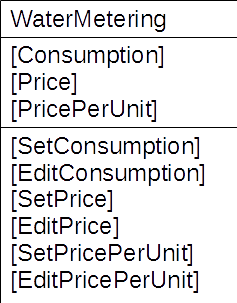
\includegraphics[width=\textwidth]{./WaterMetering.png}
    \caption{Class Diagrams for the proposed system} \label{fig:WaterMetering Class Diagram}
\end{figure}
\begin{figure}[H]
    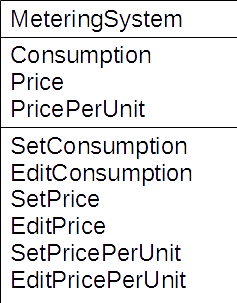
\includegraphics[width=\textwidth]{./MeteringSystem.png}
    \caption{Class Diagrams for the proposed system} \label{fig:MeteringSystem Class Diagram}
\end{figure}
\begin{figure}[H]
    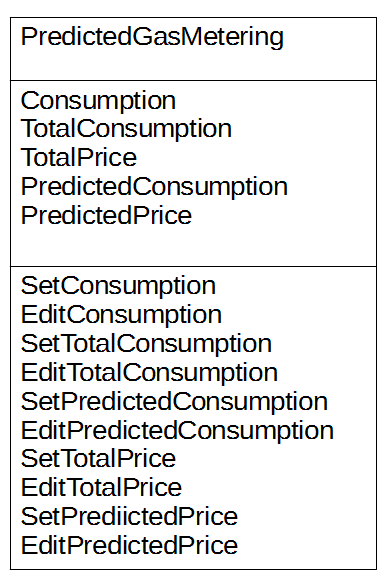
\includegraphics[width=\textwidth]{./PredictedGasMetering.png}
    \caption{Class Diagrams for the proposed system} \label{fig:PredictedGasMetering Class Diagram}
\end{figure}
\begin{figure}[H]
    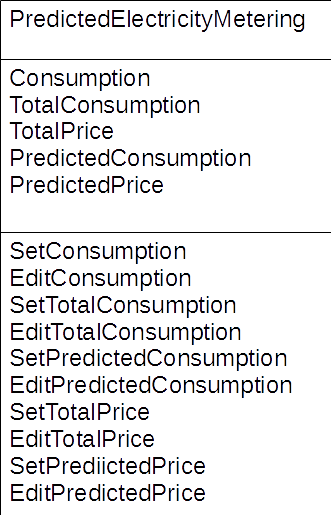
\includegraphics[width=\textwidth]{./PredictedElectricityMetering.png}
    \caption{Class Diagrams for the proposed system} \label{fig:PredictedElectricityMetering Class Diagram}
\end{figure}
\begin{figure}[H]
    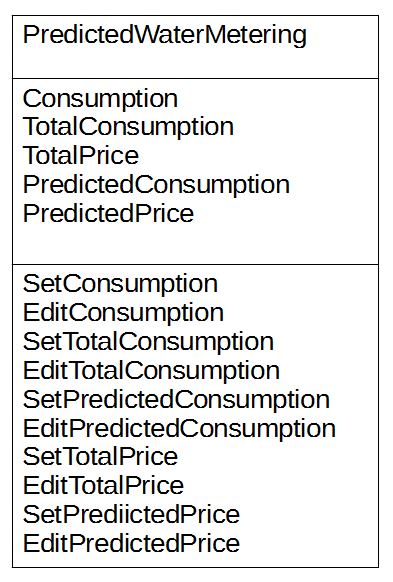
\includegraphics[width=\textwidth]{./PredictedWaterMetering.png}
    \caption{Class Diagrams for the proposed system} \label{fig:PredictedWaterMetering Class Diagram}
\end{figure}
\begin{figure}[H]
    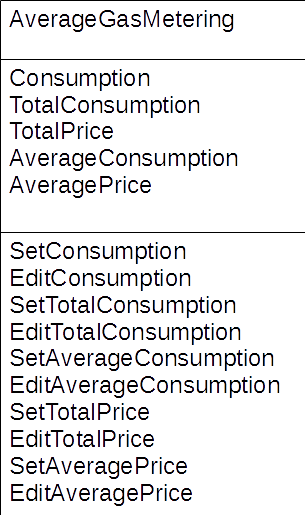
\includegraphics[width=\textwidth]{./AverageGasMetering.png}
    \caption{Class Diagrams for the proposed system} \label{fig:AverageGasMetering Class Diagram}
\end{figure}
\begin{figure}[H]
    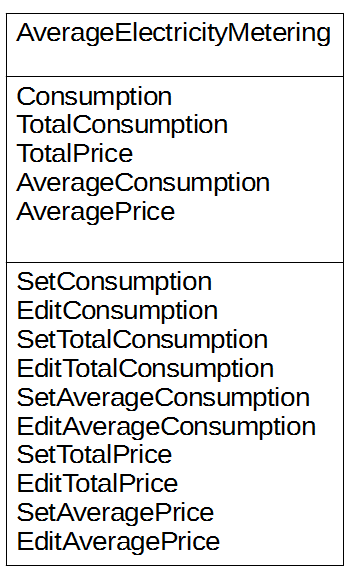
\includegraphics[width=\textwidth]{./AverageElectricityMetering.png}
    \caption{Class Diagrams for the proposed system} \label{fig:AverageElectricityMetering Class Diagram}
\end{figure}
\begin{figure}[H]
    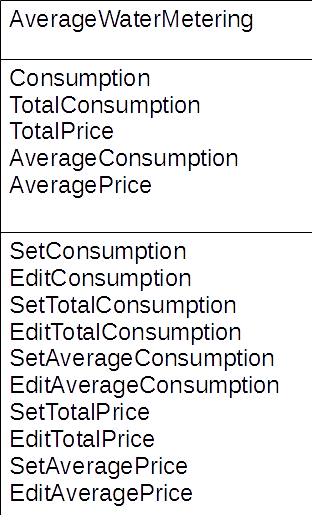
\includegraphics[width=\textwidth]{./AverageWaterMetering.png}
    \caption{Class Diagrams for the proposed system} \label{fig:AverageWaterMetering Class Diagram}
\end{figure}
\section{Other Abstractions and Graphs}

\section{Constraints}

\subsection{Hardware}
My client currently uses a laptop to do his daily work, read his emails and browse the web. He has requested that the proposed system will be able to run on this device.

The main hardware specifications of this laptop are:
\begin{itemize}
	\item 1TB Hard Drive
	\item 8GB RAM
	\item Intel Celeron Dual Core CPU
\end{itemize}
The proposed system will not have a large impact on this hardware so running on my client's laptop is not too much of a problem.
However, there are still a few hardware constraints that impact the proposed system. For example, the user interface has to be designed to work well on a display with a resolution of 1366x768 as that is the resolution of my client's laptop display and that the system will need to be able to do auto saves regularly as the laptop only has limited power available as it is powered by a battery which means that the laptop could shut down when the battery power gets too low and potentially cause data to be lost
\subsection{Software}
The proposed system will need to be designed to work on windows 8 as that is the operating system that my client uses on his laptop. In addition to that, my client has expressed that he is capable of installing any additional software on his laptop if required but he would prefer it if there isn't too much additional software required if any is at all.
\subsection{Time}
My client has not expressed any dates for when he needs the system, so the only time constraint for this will be the deadline that has been set by my teacher which is 13th February.
\subsection{User Knowledge}
My client is fairly knowledgable with computers and is experienced in using many different types of software and understands IT terms which means this is not a serious constraint on the proposed system.
\subsection{Access restrictions}
This system will only be going onto my client's laptop which only he uses, so he will be the only person who can have access to this software. However, a password will still be implemented as the database will be storing financial data which my client would prefer to keep private and this will maximise the security of the system.
\section{Limitations}

\subsection{Areas which will not be included in computerisation}
Gathering of the initial average price per unit for gas, electricity and water consumption will not be computerised as they can be gathered from the notepad and inputted into the system when needed.
\subsection{Areas considered for future computerisation}
In the future the average price per unit for gas, electricity and water consumption may be able to be computerised by working it out from the previous values that will be stored in the system from when the user inputs them.
\section{Solutions}

\subsection{Alternative solutions}
\begin{center}
\begin{tabular}{|l|p{4.5cm}|p{4.5cm}|}
	\hline
	\textbf{Solution} & \textbf{Advantages} & \textbf{Disadvantages} \\ \hline
	Spreadsheet & \begin{itemize} \item No extra software needed \item simple to use \end{itemize} & \begin{itemize} \item Can be difficult to implement \item available software may not be able to do everything the user needs \item security may not be as good as required \end{itemize} \\ \hline
	Web based system & \begin{itemize} \item no software needed to be installed \item can access from anywhere at any time with an internet connection \item easy to backup \item can be accessed by multiple people simultaneously \end{itemize} & \begin{itemize} \item can be expensive to host \item need experience of web based programming languages to implement \item harder to use \item more security methods needed due to the system constantly being online \end{itemize} \\ \hline
	Re-designing the current system & \begin{itemize} \item no computer / software needed \item low cost \item can transfer old skills \end{itemize} & \begin{itemize} \item current problems may persist \item inefficient and slow \item alot of physical storage is needed \end{itemize} \\ \hline
	System with a graphical interface & \begin{itemize} \item Easy to understand what the program is doing \item Easy to display large amounts of data \item can minimise errors by using buttons rather than text based inputs where possible \item Easy to format data \end{itemize} & \begin{itemize} \item Can take alot longer \item Can be more difficult to make the GUI \item more intense on the hardware than other solutions \end{itemize}\\ \hline
\end{tabular}
\end{center}
\subsection{Justification of chosen solution}
I have chose to implement a system with a graphical interface over the other solutions. This is because of several reasons:
\begin{itemize}
	\item I can tailor the system to be specific to my client's needs easier than with a premade spreadsheet or other software
	\item Backups can be made to the system if needed
	\item More time efficient than doing it manually
	\item More space efficient than a manual solution
\end{itemize}